\chapter{Objects of Arrays}

\begin{exercise}
The previous chapter's exercise that implemented a \java{Course} class lacks one important feature: most courses meet more than one day a week. Figure~\ref{fig.course2uml} is a revised UML diagram for an implementation of \java{Course} that solves that problem:

\begin{figure}[!h]
\begin{center}
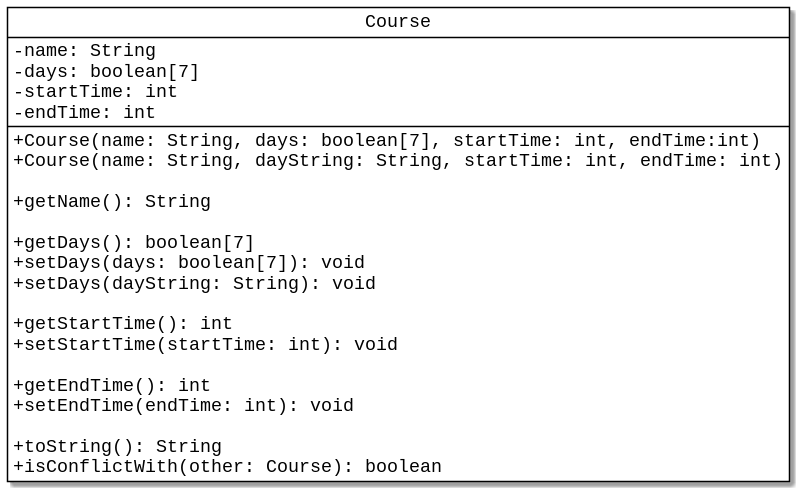
\includegraphics[scale=0.5]{figs/ch13/course.png}
\caption{UML Diagram for a Course class}
\label{fig.course2uml}
\end{center}
\end{figure}

Instead of having one day of the week, \java{Course} objects will now contain an array of seven \java{boolean} values, where \java{true} indicates that the course meets on that day. Array entry 0 corresponds to Monday, 1 to Tuesday, and so on until entry 6 for Sunday.

Notice that there are two constructors. The first one has you provide an array of booleans; the second has you provide a \java{String} that represents the days on which a course meets. This string will have the format of one or more day abbreviations separated by slashes.  The abbreviations are \java{"M"}, \java{"T"}, \java{"W"}, \java{"Th"}, \java{"F"}, \java{"Sa"}, and  \java{"Su"}.  Your constructor will translate this string into the appropriate array of \java{boolean} for the \java{days} attribute. This gives you two ways to construct a course:

\begin{code}
Course course1 = new Course("ECON 101",
   new boolean[]{true, false, true, false, true, false, false},
   915, 1045);

Course course2 = new Course("ECON101", "M/W/F", 915, 1045);
\end{code}

Similarly, the two \java{setDays} methods allow you to set the days on which a course meets by passing in array of seven \java{boolean} values or a \java{String} as described. These are equivalent:

\begin{code}
// change to Tuesday-Thursday
course1.setDays(new boolean[]{false, true, false, true,
   false, false, false});

course2.setDays("T/Th");
\end{code}

Instead of the \java{compareTo} method from the previous exercise, you will write an \java{isConflictWith} method that returns \java{true} if the days and times of the two courses overlap, \java{false} otherwise.  {\em Hint}: first, check to see if both courses have a day in common. For example, a Monday/Wednesday course and a Tuesday/Wednesday course might have a conflict. A Monday/Wednesday course cannot have a conflict with a Tuesday/Thursday course since the two courses are on different days.

If there is a day conflict, then check the times to see if they overlap. Two courses overlap if the course with the earlier start time ends after the course with the later start time begins.  Thus, a course from 0915 to 1045 overlaps with a class from 1015 to 1230.  If the end of the earlier course is the same time as the start of the later one, that is {\em not} an overlap: a class from 0915 to 1045 does not overlap a class from 1045 to 1215. (We presume that you can teleport instantly from one classroom to the other.)

Once you have the \java{Course} class written, write a test program whose \java{main} method sets up this array of courses:

\begin{tabular}{|l|l|l|l|}
\hline
Name & Days & Start Time & End Time \\ \hline
ECON 101 & M/W & 0915 & 1135 \\ \hline
PHYS 002 & Tu/Th & 1025 & 1300 \\ \hline
COMSC 079C & M & 0745 & 0930 \\ \hline
ACCTG 0063A & W/F & 1015 & 1235 \\ \hline
CHEM 001 & Tu/Th & 1700 & 1925 \\ \hline
MATH 017 & M/Tu/W/Th & 1305 & 1545 \\ \hline
ART 099 & Tu/Th & 1205 & 1335 \\ \hline
\end{tabular}

Once you have set up this array, your code will look at all the pairs of courses and display the ones that have a time conflict.

Here is what the output might look like:

\begin{stdout}
Course conflicts:
ECON 101 M/W (0915-1135) and COMSC 079C M (0745-0930)
ECON 101 M/W (0915-1135) and ACCTG 063A W/F (1015-1235)
PHYS 002 T/Th (1025-1300) and ART 099 T/Th (1205-1635)
MATH 017 M/T/W/Th (1305-1545) and ART 099 T/Th (1205-1635)
\end{stdout}

Do not duplicate the conflict information. For example, ECON 101 conflicts with COMSC 079C, so there is no need to output that COMSC 079C conflicts with ECON 101.

Your code must work for any set of courses. If there are no conflicts, then your program should output a message to that effect, for example:

\begin{stdout}
Course conflicts:
None found
\end{stdout}

\end{exercise}

\begin{exercise}
Create a \java{Competitor} class. Make a UML diagram {\em before} you start implementing the class, according to the following specifications.

A \java{Competitor} object has these private attributes:

\begin{itemize}
\item A \java{name}, which is a \java{String}.
\item A \java{team}, which is a \java{String} that can have the value \java{"Green"} or \java{"Orange"}.
\item An array of \java{scores}, which is an array of three \java{int} values that gives the competitor's score in each of three games. A value of -1 means that the competitor did not take part in the game.
\end{itemize}

Write a constructor and getters and setters for each of the attributes. Write a \java{toString} method that displays a competitor's information. (I have deliberately left this open-ended. Use your judgment as to what the return value should look like.)

Now that you have the \java{Competitor} class, write a program whose \java{main} method sets up the following array of competitors:

\begin{tabular}{|l|l|r|r|r|}
\hline
Name & Team & First Game & Second Game & Third Game \\ \hline
Tom & Orange & 5 & 17 & 22 \\ \hline
Joe & Green & 3 & 14 & 22 \\ \hline
Maria & Green & 6 & 18 & 21 \\ \hline
Fred & Orange & 15 & -1 & 23 \\ \hline
Carlos & Orange & 17 & 15 & 24 \\ \hline
Phuong & Green & 7 & 19 & 21 \\ \hline
Enrique & Green & 3 & 16 & 20 \\ \hline
Nancy & Orange & 9 & 12 & 24 \\ \hline
\end{tabular}

Then compute and print:

\begin{itemize}
\item The average score for every person in the array
\item The average score for each game
\item The average score for each team
\end{itemize}

\end{exercise}

\begin{exercise}
This exercise will familiarize you with \java{ArrayList}s. You will use the \java{Person} class that has been written for you and is available in the code repository that accompanies this book. Figure~\ref{fig.personuml} shows the UML diagram for the class.

\begin{figure}[!h]
\begin{center}
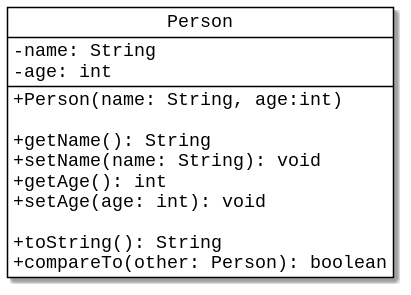
\includegraphics[scale=0.5]{figs/ch13/person.png}
\caption{UML Diagram for the Person class}
\label{fig.personuml}
\end{center}
\end{figure}

The \java{compareTo} method compares the names; if they are equal, it compares the ages. In this exercise, we won't allow duplicate names, but the code is written to be general enough to work in other applications.

Write a program that creates an \java{ArrayList<Person>} and repeatedly asks users to either:

\begin{itemize}
\item Add a name and age to the list if it isn't already there.
\item Remove a name (and its age) from the list if it is in the list.
\item Change the age for a person if the person is in the list.
\item Finish
\end{itemize}

When the user finishes, the program sorts the \java{ArrayList} {\em by age}, which means you will {\em not} use the \java{compareTo} method, which would sort them by name. It then prints the sorted list of users:

\begin{stdout}
A)dd, R)emove, C)hange age, F)inish: A
Enter name: Joe
Enter age: 2r
Please use digits for your answer.
Enter age: 24
A)dd, R)emove, C)hange age, F)inish: A
Enter name: Marta 
Enter age: 47
A)dd, R)emove, C)hange age, F)inish: a
Enter name: Douglas
Enter age: 33
A)dd, R)emove, C)hange age, F)inish: A
Enter name: Vinh
Enter age: 18
A)dd, R)emove, C)hange age, F)inish: a
Enter name: Vinh
Vinh is already in the list.
A)dd, R)emove, C)hange age, F)inish: r
Enter name: Josephine
Josephine is not in the list.
A)dd, R)emove, C)hange age, F)inish: R
Enter name: Douglas
Removed Douglas.
A)dd, R)emove, C)hange age, F)inish: C
Enter name: Vinh
Enter age: 19
Vinh is now 19 years old.
A)dd, R)emove, C)hange age, F)inish: F

People sorted by age:
Vinh (19)
Joe (24)
Marta (47)
\end{stdout}

Your program should allow the commands to be input in either upper or lower case. As in the sample output, it should produce appropriate error messages if the user tries to add a duplicate name, remove a non-existent name, or give an invalid command.

\end{exercise}


